\documentclass[letterpaper,12pt]{article}
\usepackage{dgjournal}          
\usepackage{mathptmx}
\usepackage{graphicx} % Allows use of width and scale options for \includegraphics
\usepackage[authoryear,comma,longnamesfirst,sectionbib]{natbib} 
%% The lineno packages adds line numbers. Start line numbering with
%% \begin{linenumbers}, end it with \end{linenumbers}. Or switch it on
%% for the whole article with \linenumbers after \end{frontmatter}.
\usepackage{lineno}


\begin{document}

\linenumbers % Turns on line numbering

%% Do NOT include any frontmatter information; including the title, author names,
%% institutes, acknowledgments and title footnotes (author information, funding
%% sources, etc.). Start the document with the first section or paragraph of
%% the article.

%%%%%%%%%%%%%%%%%%%%%%%%%%%%%%%
\section*{Abstract}
%%%%%%%%%%%%%%%%%%%%%%%%%%%%%%%


%%%%%%%%%%%%%%%%%%%%%%%%%%%%%%%
\section{Introduction}
%%%%%%%%%%%%%%%%%%%%%%%%%%%%%%%


%%%%%%%%%%%%%%%%%%%%%%%%%%%%%%%
\section{Sources of Data}
%%%%%%%%%%%%%%%%%%%%%%%%%%%%%%%

**** Caleb complete this section ****


%%%%%%%%%%%%%%%%%%%%%%%%%%%%%%%
\section{Basic model (without energy and capital stock)}
%%%%%%%%%%%%%%%%%%%%%%%%%%%%%%%

The model is adapted from the longwave growth model of \citet{Jones:2001wn}. **** Caleb update this section ****


%++++++++++++++++++++++++++++++
\subsection{Basic model development}
%++++++++++++++++++++++++++++++

\begin{figure} \label{fig:ModelWithoutEnergy}
  \begin{center}
    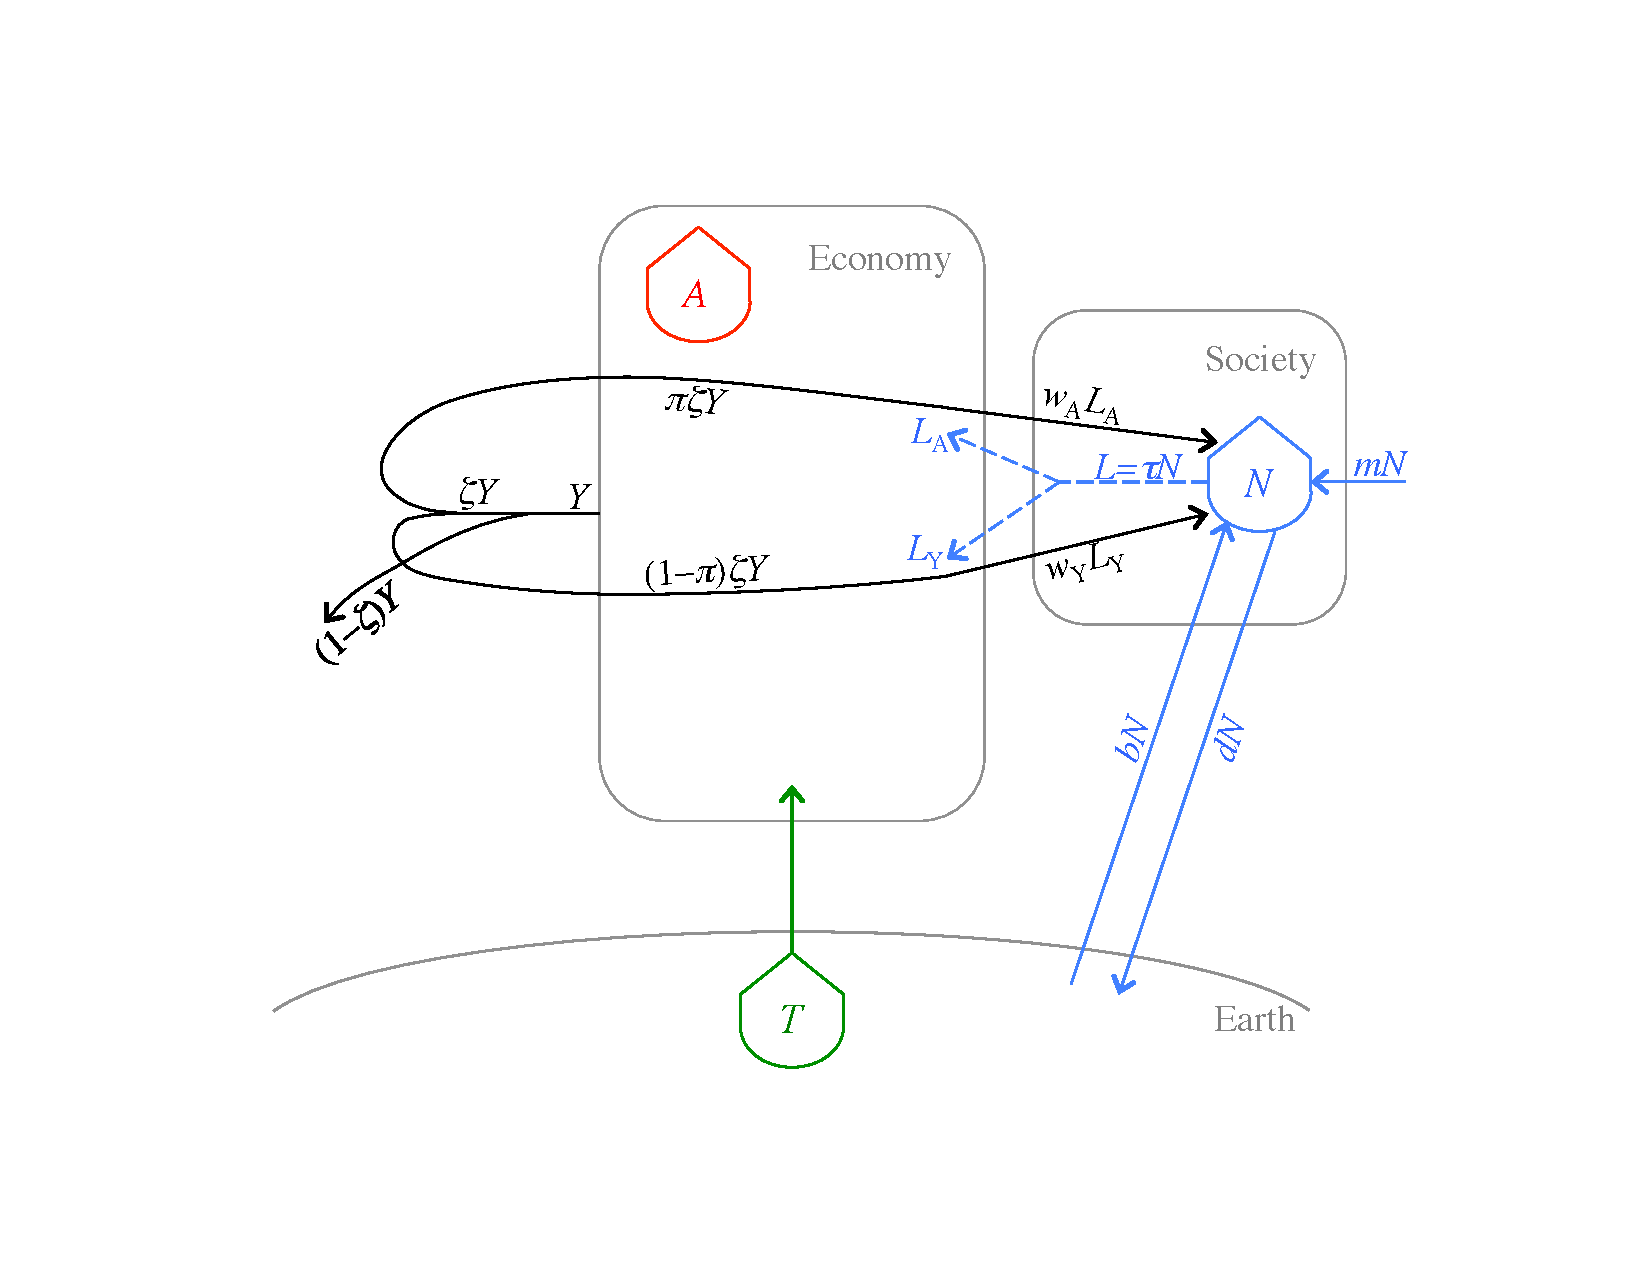
\includegraphics[width=\textwidth]{figure_other/ModelWithoutEnergy.pdf}
    \caption{Dynamic model without energy.}
  \end{center}
\end{figure}

For \citet{Jones:2001wn}, economic production is given by

\begin{equation} \label{eq:Jones_production_function}
	y_\mathrm{t} = a_\mathrm{t} ^\sigma l_\mathrm{Y,t} ^\beta t_\mathrm{t} ^{1-\beta} \epsilon_\mathrm{t}
\end{equation}

\noindent where $a_\mathrm{t}$ is the indexed stock of ideas, $l_\mathrm{Y,t}$ is indexed labor in the goods producing sector, $t_\mathrm{t}$ is indexed land (always 1.0), and $\epsilon_\mathrm{t}$ is an exogenous shock parameter. 

Lowercase variables represent unitless indexed variables. The indexed factors of production ($a$, $l$, and $t$) at time $\mathrm{t}$ are non-dimensionalized by indexing relative to a base year (subscript ``0''):

\begin{equation} \label{eq:index_y}
	y_\mathrm{t} \equiv \frac{Y_\mathrm{t}}{Y_\mathrm{0}}
\end{equation}

\begin{equation} \label{eq:index_a}
	a_\mathrm{t} \equiv \frac{A_\mathrm{t}}{A_\mathrm{0}}
\end{equation}

\begin{equation} \label{eq:index_l}
	l_\mathrm{Y,t} \equiv \frac{L_\mathrm{Y,t}}{L_\mathrm{Y,0}}
\end{equation}

\begin{equation} \label{eq:index_t}
	t_\mathrm{t} \equiv \frac{T_\mathrm{t}}{T_\mathrm{0}}
\end{equation}

\noindent with $Y$ representing economic output (in \$/year), $A$ representing the stock of knowledge and ideas (in ideas), $L_\mathrm{Y}$ representing labor in the production sector (in workers/year), and $T$ representing the stock of available land ($\mathrm{m}^2$).

Our model for preferences between consumption and childrearing is based on the utility function from \citet{Jones:2001wn}:

\begin{equation} \label{eq:utility_function}
	u(c_\mathrm{t}, b_\mathrm{t}) = u_\mathrm{c} + u_\mathrm{b} = \frac{1-\mu}{1-\gamma} \left(\frac{k_\mathrm{c} \tilde c_\mathrm{t}}{U_\mathrm{c,0}} \right)^{1-\gamma} + \frac{\mu}{1-\eta} \left(\frac{k_\mathrm{b} \tilde b_\mathrm{t}}{U_\mathrm{b,0}} \right)^{1-\eta}
\end{equation}

\noindent where $\mu$, $\gamma$, and $\eta$ are dimensionless parameters having values between 0 and 1; $k_\mathrm{c}$ and $k_\mathrm{b}$ represent the utility an individual obtains per unit consumption or birth (in units of utils/\$ and utils/birth, respectively); and $U_{\mathrm{c,0}}$ and $U_{\mathrm{b,0}}$ are the utility derived from consumption and childrearing in the first year of the simulation, respectively (in units of utils/year). The variable $\tilde c_\mathrm{t}$ is the amount of the individual's consumption in \$/year-person ****** per worker or per capita? ****** and $\tilde b_\mathrm{t}$ is the number of births in births/year-person ***** per worker or per capita? *******. $\tilde c_\mathrm{t}$ represents the amount of consumption above subsistence level ($\bar c$ in \$/year-person ***** per worker or per capita? *******) and $\tilde b_\mathrm{t}$ represents the amount of births above some long-run birth rate ($\bar b$, in births/year-capita). $u_\mathrm{c}$ and $u_\mathrm{b}$ are the utilities obtained from consumption and births, represented by the left and right terms respectively in the last part of the equation.

\begin{equation} \label{eq:c_tilde}
	\tilde c_\mathrm{t} \equiv c_\mathrm{t} - \bar c
\end{equation}

\begin{equation} \label{eq:b_tilde}
	\tilde b_\mathrm{t} \equiv b_\mathrm{t} - \bar b
\end{equation}

The first order condition on the utility function indicates that a person will obtain equal incremental utility from spending additional time consuming or rearing children:

\begin{equation} \label{eq:first_order_condition_def}
	\frac{\partial u_{c}}{\partial \tau} = \frac{\partial u_{b}}{\partial \tau}
\end{equation}

\noindent The first order condition simplifies to 

\begin{equation} \label{eq:first_order_condition_simplified}
	\frac{\partial u/ \partial\tilde b}{\partial u/ \partial\tilde c} = \frac{w_\mathrm{t}}{\alpha},
\end{equation}

\noindent where $w_\mathrm{t}$ is the wage rate that a worker is paid (in \$/year-person ***** per worker or per capita? *******) and $\alpha$ is a birth efficiency (in births/year-capita). [**** Caleb: notice that I'm using ``per capita'' in several places. Is that appropriate? I think we want to avoid ``per person'' wherever possible, preferring instead ``per capita'' or ``per worker.'' --Prof. Heun ****] $w_\mathrm{t}$ and $\alpha$ come from the time constraints in the economy. These time constraints are given by:

\begin{equation}\label{eq:pop_work}
	L = \tau_\mathrm{t} N
\end{equation}

\begin{equation} \label{eq:consumption_constraint}
	c_\mathrm{t} = w_\mathrm{t} \tau_\mathrm{t}
\end{equation}

\begin{equation} \label{eq:birth_constraint}
	b_\mathrm{t} = \alpha (1-\tau_\mathrm{t})
\end{equation}

\noindent where $\tau$ is a number between 0 and 1 representing the fraction of available time that people spend on labor (unitless), $N$ is the total population (in persons), and $L$ is the total amount of available labor in the economy (in persons ***** in workers? *******). So, $(1-\tau)$ represents the fraction of available time spent on childrearing.

Applying the first order condition (Equation \ref{eq:first_order_condition_simplified}) and including time constraints yields an equation that describes preferences for consumption and childrearing:

\begin{equation} \label{eq:FOC_and_time_constraints}
	\frac{1}{\alpha \mu} \frac{U_\mathrm{b,0}}{k_\mathrm{b}} \left( \frac{k_\mathrm{b}}{U_\mathrm{b,0}} \tilde b_\mathrm{t} \right) ^{\eta} 
	= \frac{1}{w_\mathrm{t}(1-\mu)} \frac{U_\mathrm{c,0}}{k_\mathrm{c}}  \left( \frac{k_\mathrm{c}}{U_\mathrm{c,0}} \tilde c_\mathrm{t} \right)^\gamma .
\end{equation}

Labor is split between two sectors; one devoted to innovation and producing new ideas ($A$) and one devoted to producing goods ($Y$). The split between these sectors is based on the wages paid to each as shown in the equations below:

\begin{equation} \label{eq:knowledge_comp}
	w_\mathrm{A,t} L_\mathrm{A,t} = \pi_\mathrm{t} Y_\mathrm{t}
\end{equation}

\begin{equation} \label{eq:labor_comp}
	w_\mathrm{Y,t} L_\mathrm{Y,t} = (1-\pi) Y_\mathrm{t}
\end{equation}

\noindent where $w_\mathrm{A,t}$ and $w_\mathrm{Y,t}$ are the wages paid to workers in the knowledge and goods producing sectors respectively (in \$/person-year ***** per worker or per capita? *******), and $L_\mathrm{A,t}$ and $L_\mathrm{Y,t}$ represent the number of workers employed by each of the sectors (in persons/year ***** workers/year or capita/year? *******). The total labor supply is constrained as the sum of the two sectors.

\begin{equation} \label{labor_supply}
	L_\mathrm{t} = L_\mathrm{A,t} + L_\mathrm{Y,t}
\end{equation}

The two labor supplies can also indexed when necessary.

\begin{equation}
	l_\mathrm{Y,t} \equiv \frac{L_\mathrm{Y,t}}{L_\mathrm{Y,0}}
\end{equation}

\begin{equation}
	l_\mathrm{A,t} \equiv \frac{L_\mathrm{A,t}}{L_\mathrm{A,0}}
\end{equation}

In equilibrium, it is expected that the wages will be equal.

\begin{equation} \label{eq:wage_equality}
	w_\mathrm{A,t} = w_\mathrm{Y,t} = w_\mathrm{t}
\end{equation}

The dimensionless variable $\pi_\mathrm{t}$ is the fraction of the economy's total output ($Y_\mathrm{t}$) that is devoted to compensating inventors. The wage equality allows $\pi_\mathrm{t}$ to be directly proportional to the fraction of the total employed population working in the knowledge sector in static equilibrium.

\begin{equation} \label{eq:pi}
	\pi_\mathrm{t} = \frac{L_\mathrm{A,t}}{L_\mathrm{t}}
\end{equation}

Two differential equations describe the growth of knowledge and population over time in the production function (Equation \ref{eq:Jones_production_function}), because population directly affects the labor force. The rate of change in the indexed stock of knowledge ($a_{\mathrm{t}}$) is given by

\begin{equation} \label{eq:da_dt}
	\frac{da}{dt} = \delta l_\mathrm{A,t}^\lambda a_\mathrm{t}^\phi,
\end{equation}

\noindent where $\delta$, $\lambda$, and $\phi$ are constants, $l_\mathrm{A,t}$ is the indexed labor in the knowledge sector of the economy, and $a_\mathrm{t}$ is the indexed stock of ideas.

The rate of change of indexed population ($n$) is a function of birth and mortality rates ($b$ and $d$ in births/year-capita and deaths/year-capita, respectively):

\begin{equation} \label{eq:dn_dt}
	\frac{dn}{dt} = b_\mathrm{t} n_\mathrm{t} - d_\mathrm{t} n_\mathrm{t},
\end{equation}

\noindent where $b_\mathrm{t}$ is the birth rate from Equation \ref{eq:utility_function}, $n_\mathrm{t}$ is the indexed population, and $d_\mathrm{t}$ is the mortality rate in deaths/person-year ***** per worker or per capita? *******. The mortality rate is determined from a fit of historical mortality rate data \citep{Jones:2001wn} and is given by

\begin{equation} \label{eq:mortality_rate}
	d_\mathrm{t} = \frac{1}{\omega_\mathrm{1} z_\mathrm{t}^{\omega_\mathrm{2}} + \omega_\mathrm{3} z_\mathrm{t}} + \bar d,
\end{equation}

\noindent where $d_\mathrm{t}$ is the mortality rate and $\bar d$ is the long-run mortality rate, both in units of deaths/year-person ***** per worker or per capita? *******. $\omega_\mathrm{1}$, $\omega_\mathrm{2}$, and $\omega_\mathrm{3}$ are fitted parameters. The ratio of consumption to the subsistence level is given by $z_\mathrm{t}$:

\begin{equation} \label{eq:z}
	z_\mathrm{t} = \frac{c_\mathrm{t}}{\bar c} - 1, 
\end{equation}

\noindent which is an indicator of the mortality rate through Equation \ref{eq:mortality_rate}.

%++++++++++++++++++++++++++++++
\subsection{Tuning: basic model}
%++++++++++++++++++++++++++++++

**** Caleb discuss the process you used to tune the model. ****

%++++++++++++++++++++++++++++++
\subsection{Results: basic model}
%++++++++++++++++++++++++++++++

**** MKH to develop graphs and other results based on Caleb's existing work ****


%%%%%%%%%%%%%%%%%%%%%%%%%%%%%%%%
\section{Enhanced model (with energy and capital stock)}
%%%%%%%%%%%%%%%%%%%%%%%%%%%%%%%%

%++++++++++++++++++++++++++++++
\subsection{Enhanced model development}
%++++++++++++++++++++++++++++++

We now enhance the basic model with both energy flows and capital stock.

\begin{figure} \label{fig:ModelWithEnergy}
  \begin{center}
    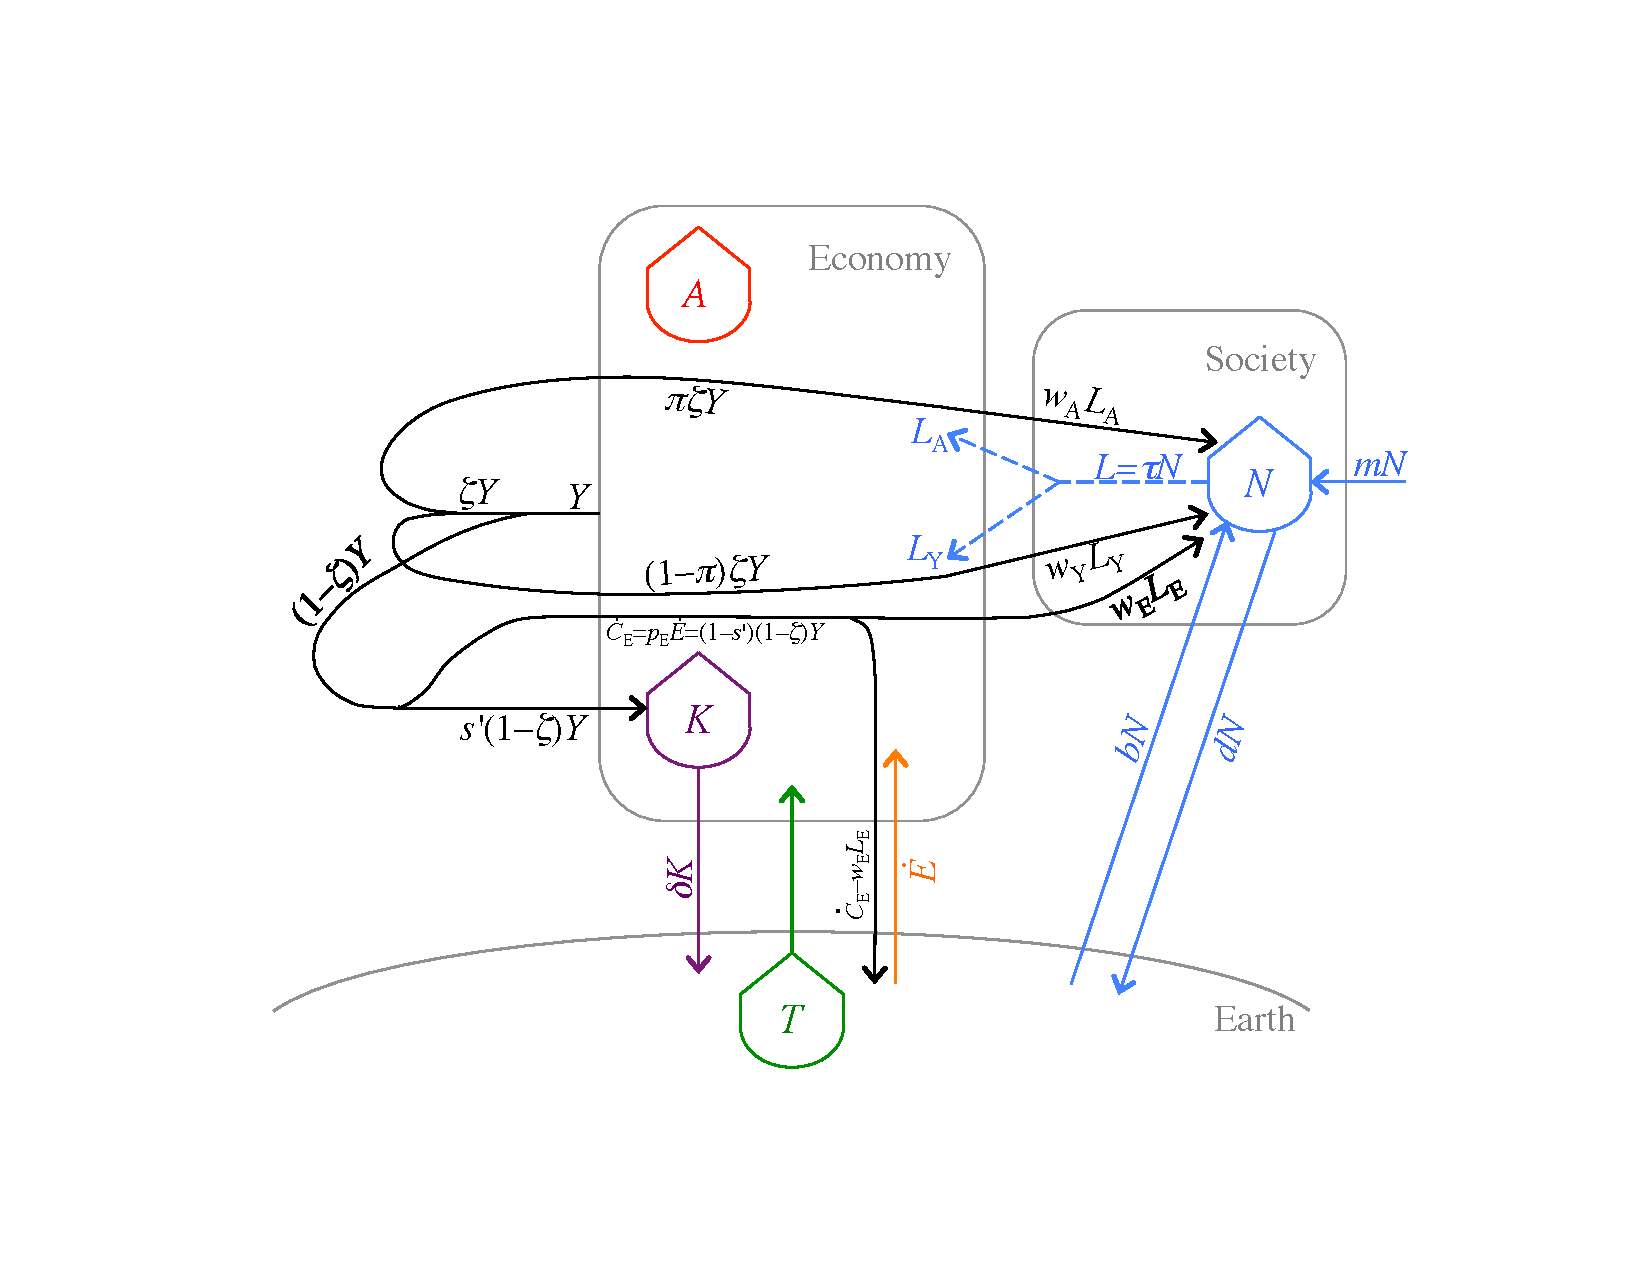
\includegraphics[width=\textwidth]{figure_other/ModelWithEnergy.pdf}
    \caption{Dynamic model with energy.}
  \end{center}
\end{figure}

%++++++++++++++++++++++++++++++
\subsection{Tuning: enhanced model}
%++++++++++++++++++++++++++++++

**** Caleb: discuss the process you used to tune the enhanced model. ****

%++++++++++++++++++++++++++++++
\subsection{Results: enhanced model}
%++++++++++++++++++++++++++++++

**** MKH to develop graphs and other results based on Caleb's existing work ****


%%%%%%%%%%%%%%%%%%%%%%%%%%%%%%%
\section{Implications}
%%%%%%%%%%%%%%%%%%%%%%%%%%%%%%%

%%%%%%%%%%%%%%%%%%%%%%%%%%%%%%%
\section{Conclusion}
%%%%%%%%%%%%%%%%%%%%%%%%%%%%%%%


%%%%%%%%%%%%%%%%%%%%%%%%%%%%%%%
%% Bibliography (via BibTeX)
%%%%%%%%%%%%%%%%%%%%%%%%%%%%%%%
\bibliographystyle{DeGruyter}
\bibliography{ReeseHeunJournalPaper}

\end{document}